
\documentclass{article}
\usepackage{graphicx}
\usepackage[margin=1in]{geometry}
\title{Stock Report: AAPL}
\author{Jack Massey}
\date{\today}

\begin{document}
\maketitle

\section*{Summary}
\begin{itemize}
    \item Latest Close Price: 199.74 USD
    \item Growth (1Y): 20.24\%
    \item Volatility: 0.0206
    \item P/E Ratio: 31.76
    \item Market Cap: 3.00 Trillion
\end{itemize}

\section*{Today's Data}
\begin{tabular}{lr}\textbf{Metric} & \textbf{Value} \\
\hline
Open & 196.12 \\
High & 201.59 \\
Low & 195.97 \\
Close & 199.74 \\
Volume & 52,660,200.00 \\
Dividends & 0.00 \\
Stock Splits & 0.00 \\
Daily Return & 0.03 \\
50MA & 220.46 \\
200MA & 227.60 \\
EMA12 & 198.71 \\
EMA26 & 205.74 \\
MACD & -7.03 \\
Signal & -7.87 \\
Histogram & 0.84 \\
RSI & 40.27 \\
20MA & 203.90 \\
20STD & 15.66 \\
Upper Band & 235.21 \\
Lower Band & 172.58 \\
\end{tabular}

\section*{Bollinger Bands Chart}
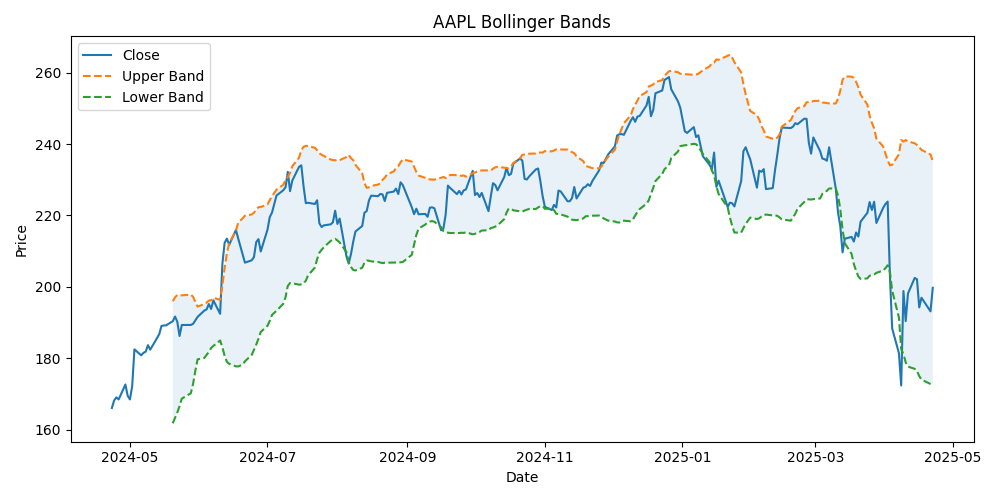
\includegraphics[width=\textwidth]{bollinger_plot.png}

\section*{Insights}
Based on current indicators, AAPL shows a trend with recent Bollinger Bands reflecting volatility thresholds. Consider analyzing MACD and RSI for confirmation signals.

\end{document}
